
%% bare_jrnl.tex
%% V1.4b
%% 2015/08/26
%% by Michael Shell
%% see http://www.michaelshell.org/
%% for current contact information.
%%
%% This is a skeleton file demonstrating the use of IEEEtran.cls
%% (requires IEEEtran.cls version 1.8b or later) with an IEEE
%% journal paper.
%%
%% Support sites:
%% http://www.michaelshell.org/tex/ieeetran/
%% http://www.ctan.org/pkg/ieeetran
%% and
%% http://www.ieee.org/

%%*************************************************************************
%% Legal Notice:
%% This code is offered as-is without any warranty either expressed or
%% implied; without even the implied warranty of MERCHANTABILITY or
%% FITNESS FOR A PARTICULAR PURPOSE!
%% User assumes all risk.
%% In no event shall the IEEE or any contributor to this code be liable for
%% any damages or losses, including, but not limited to, incidental,
%% consequential, or any other damages, resulting from the use or misuse
%% of any information contained here.
%%
%% All comments are the opinions of their respective authors and are not
%% necessarily endorsed by the IEEE.
%%
%% This work is distributed under the LaTeX Project Public License (LPPL)
%% ( http://www.latex-project.org/ ) version 1.3, and may be freely used,
%% distributed and modified. A copy of the LPPL, version 1.3, is included
%% in the base LaTeX documentation of all distributions of LaTeX released
%% 2003/12/01 or later.
%% Retain all contribution notices and credits.
%% ** Modified files should be clearly indicated as such, including  **
%% ** renaming them and changing author support contact information. **
%%*************************************************************************


% *** Authors should verify (and, if needed, correct) their LaTeX system  ***
% *** with the testflow diagnostic prior to trusting their LaTeX platform ***
% *** with production work. The IEEE's font choices and paper sizes can   ***
% *** trigger bugs that do not appear when using other class files.       ***                          ***
% The testflow support page is at:
% http://www.michaelshell.org/tex/testflow/



\documentclass[journal,10pt]{IEEEtran}
%
% If IEEEtran.cls has not been installed into the LaTeX system files,
% manually specify the path to it like:
% \documentclass[journal]{../sty/IEEEtran}





% Some very useful LaTeX packages include:
% (uncomment the ones you want to load)


% *** MISC UTILITY PACKAGES ***
%
%\usepackage{ifpdf}
% Heiko Oberdiek's ifpdf.sty is very useful if you need conditional
% compilation based on whether the output is pdf or dvi.
% usage:
% \ifpdf
%   % pdf code
% \else
%   % dvi code
% \fi
% The latest version of ifpdf.sty can be obtained from:
% http://www.ctan.org/pkg/ifpdf
% Also, note that IEEEtran.cls V1.7 and later provides a builtin
% \ifCLASSINFOpdf conditional that works the same way.
% When switching from latex to pdflatex and vice-versa, the compiler may
% have to be run twice to clear warning/error messages.






% *** CITATION PACKAGES ***
%
%\usepackage{cite}
% cite.sty was written by Donald Arseneau
% V1.6 and later of IEEEtran pre-defines the format of the cite.sty package
% \cite{} output to follow that of the IEEE. Loading the cite package will
% result in citation numbers being automatically sorted and properly
% "compressed/ranged". e.g., [1], [9], [2], [7], [5], [6] without using
% cite.sty will become [1], [2], [5]--[7], [9] using cite.sty. cite.sty's
% \cite will automatically add leading space, if needed. Use cite.sty's
% noadjust option (cite.sty V3.8 and later) if you want to turn this off
% such as if a citation ever needs to be enclosed in parenthesis.
% cite.sty is already installed on most LaTeX systems. Be sure and use
% version 5.0 (2009-03-20) and later if using hyperref.sty.
% The latest version can be obtained at:
% http://www.ctan.org/pkg/cite
% The documentation is contained in the cite.sty file itself.






% *** GRAPHICS RELATED PACKAGES ***
%
\ifCLASSINFOpdf
  % \usepackage[pdftex]{graphicx}
  % declare the path(s) where your graphic files are
  % \graphicspath{{../pdf/}{../jpeg/}}
  % and their extensions so you won't have to specify these with
  % every instance of \includegraphics
  % \DeclareGraphicsExtensions{.pdf,.jpeg,.png}
\else
  % or other class option (dvipsone, dvipdf, if not using dvips). graphicx
  % will default to the driver specified in the system graphics.cfg if no
  % driver is specified.
  % \usepackage[dvips]{graphicx}
  % declare the path(s) where your graphic files are
  % \graphicspath{{../eps/}}
  % and their extensions so you won't have to specify these with
  % every instance of \includegraphics
  % \DeclareGraphicsExtensions{.eps}
\fi


% correct bad hyphenation here
\hyphenation{op-tical net-works semi-conduc-tor}
\let\chapter\section
\usepackage{amsmath}
\newtheorem{thm}{Theorem}
\newtheorem{prop}[thm]{Proposition}
\allowdisplaybreaks[4]
\usepackage{graphicx}
\usepackage{caption}
\usepackage{subfigure}
\usepackage{multirow}
\usepackage{caption}
\usepackage{amssymb}
\usepackage{chngpage}
\usepackage{array}
%\usepackage{algorithm}
%\usepackage{algorithmic}
\usepackage[ruled,boxed,linesnumbered]{algorithm2e}
%\usepackage{hyperref}
\usepackage{bm}
\usepackage{mathrsfs}
\usepackage{leftidx}
\usepackage{authblk}
\usepackage{booktabs}
\usepackage{tabularx}
\usepackage{threeparttable}
\usepackage[square, comma, sort&compress, numbers]{natbib}
\captionsetup{font={small}}
\usepackage{color}
\setcounter{secnumdepth}{3}
\usepackage{setspace}
\usepackage{float}
\newcommand*{\TitleFont}{%
      %\usefont{\encodingdefault}{\rmdefault}{b}{n}%
      \fontsize{22}{27.5}%
      \selectfont}
\usepackage{natbib}
\begin{document}

% paper title
% Titles are generally capitalized except for words such as a, an, and, as,
% at, but, by, for, in, nor, of, on, or, the, to and up, which are usually
% not capitalized unless they are the first or last word of the title.
% Linebreaks \\ can be used within to get better formatting as desired.
% Do not put math or special symbols in the title.
\title{\TitleFont Joint Power-Rate-Slot Resource Allocation in Energy Harvesting-Powered Wireless Body Area Networks}
%Energy-aware Resource Allocation in EH-powered D2D Communications underlaying Cellular Networks}
%Efficient Resource Allocation in Energy-Harvesting powered D2D Communications underlay Cellular Networks: A Space Matching approach
%
%
% author names and IEEE memberships
% note positions of commas and nonbreaking spaces ( ~ ) LaTeX will not break
% a structure at a ~ so this keeps an author's name from being broken across
% two lines.
% use \thanks{} to gain access to the first footnote area
% a separate \thanks must be used for each paragraph as LaTeX2e's \thanks
% was not built to handle multiple paragraphs
%

\author{Zhiqiang~Liu,~\IEEEmembership{Student Member, IEEE},
        Bin~Liu,~\IEEEmembership{Member, IEEE},
        and~Chang~Wen~Chen,~\IEEEmembership{Fellow,~IEEE}% <-this % stops a space
\thanks{Zhiqiang Liu is with the Key Laboratory of Electromagnetic Space Information, Chinese Academy of Sciences, Department of Electrical Engineering and Information Science, University of Science and Technology of China, Hefei 230027, China (e-mail: lzhq28@mail.ustc.edu.cn).}% <-this % stops a space
\thanks{Bin Liu is with the Key Laboratory of Electromagnetic Space Information, Chinese Academy of Sciences, School of Information and Technology, University of Science and Technology of China, Hefei 230027, China (e-mail: flowice@ustc.edu.cn).}
\thanks{Chang Wen Chen is with Department of Computer Science and Engineering, University at Buffalo, State University of New York, New York 002837, USA (e-mail: chencw@buffalo.edu).}}






% make the title area
\maketitle
 
% As a general rule, do not put math, special symbols or citations
% in the abstract or keywords.
\begin{abstract}
 
Wireless body area network (WBAN) has become a promising network for continuous health monitoring of various diseases. 
The limited energy of sensors in WBAN cannot support the long term work with the high requirements of Quality of Service (QoS) for health applications. 
Energy harvesting (EH)-powered WBAN, which can provide uninterrupted work, has attracted more attention from both macadamia and industry. 
However, the time-varying and heterogeneous EH states of different sensors  become an important factor when designing the resource allocation schemes in EH-powered WBAN.
In this paper, we propose a novel two-phase resource allocation scheme, which optimizes the allocation of transmission power, source rate and slots to improve the QoS performance of EH-powered WBAN. In the first phase, we analysis the relationship between the QoS performance and the source rate for satisfying the Energy Neutral Operation (ENO), and then a joint Power-Rate Control Scheme (PRCS) is proposed to optimize the source rate and transmission power for ensuring the long-term QoS performance based on the statistical properties of EH. 
Moreover, we design a QoS Aware Slot Allocation Scheme (QASAS) to dynamically adjust the time slot allocation to cope with the time-varying EH states for obtaining better short-term QoS performance in the second phase.
Finally, numerical simulation results demonstrate that the proposed joint Power-Rate-Slot resource allocation of EH-powered WBAN can effectively exploit the time-varying EH to improve both long-term and short-term QoS performance, and .


\end{abstract}

% Note that keywords are not normally used for peerreview papers.
\begin{IEEEkeywords}
 energy harvesting, resource allocation, wireless body area network (WBAN).
\end{IEEEkeywords}



% For peer review papers, you can put extra information on the cover
% page as needed:
% \ifCLASSOPTIONpeerreview
% \begin{center} \bfseries EDICS Category: 3-BBND \end{center}
% \fi
%
% For peerreview papers, this IEEEtran command inserts a page break and
% creates the second title. It will be ignored for other modes.
\IEEEpeerreviewmaketitle



\section{Introduction}

this is introduction


\section{Related works}
This is related works

\section{System model}
This is system model
\subsection{Energy Consumption Model}

\subsection{Energy Harvesting Model}

\section{Long-term Power-Rate Control Scheme}

\subsection{Relationship between Source Rate and Uninterrupted Lifetime}

\subsection{Join Power and Source Rate Optimal Allocation}

\subsection{Optimal Analytical Solution}

\subsection{Soure Rate Configuration}

\section{Short-term QoS Aware Slot Allocation Scheme}

\subsection{Energy Harvesting Process Analysis}

\subsection{Node state evaluation}

\subsection{Slot Allocation Scheme for Energy-Sufficient Nodes}

\subsection{Slot Allocation Scheme for Energy-Constraint Nodes}

\section{Simulation results}

\subsection{Simulation Setup}

\subsection{Simulation Results of Power-Rate-Slot Control Schemes}

\subsection{The Influence of Different EH Efficiencies on Performance}

\subsection{The Influence of Different Mean of Shadowing on Performance}





%%%
%%%
%%%\section{Related works}
%%%
%%%\subsection{Related works}
%%%Some related researches
%%%
%%%
%%%\subsection{Motivation}
%%%
%%%
%%%\subsection{Contributions}
%%%In this study, we investigate the resource allocation schemes in terms of the spectrum resource matching and the power allocation under a single EH-DCCN. In the EH-DCCN, D2D pairs powered by EH module are allowed to reuse the CUs' uplink spectrum resource to transmit their local data. Thus, the key contributions of this paper can be expressed as three aspects:
%%%\begin{itemize}
    %%%\item Firstly, this work is the first to .
    %%%\item Subsequently, two algorithms .
    %%%\item As a consequence, we provide .
%%%\end{itemize}
%%%
%%%
%%%\section{Network Model and Problem Statement} \label{sec:network_model}
%%%In this section, 
%%%
%%%\subsection{Scenario, node and transmission model}
%%%
%%%\subsection{Energy model}
%%%In this scenario, each EH-DP uses the harvested energy to transmit their local data. For the $d_j$-th EH-DP, $E_{d_j}^t$ units of energy can be harvested in the $t$-th time slot where $E_{d_j}^t \ge 0$. $\left\{ {E_{{d_j}}^1,E_{{d_j}}^2, \ldots ,E_{{d_j}}^t, \ldots ,E_{{d_j}}^T} \right\}$ is the time sequence of harvested energy in $T$ time slots. 
%%%\subsection{Mathematic model}
%%%optimization problem
%%%
%%%\subsection{Problem analysis}
%%%
%%%
%%%\section{Algorithms design} \label{sec:algorithms_design}
%%%In this section, two algorithms are explained at first, and the computational complexity of the two algorithms is elaborated in the later.
%%%\subsection{Outer approximation algorithm}
 %%%
%%%
%%%\subsection{Energy-aware space matching algorithm}
%%%
%%%\newtheorem{corollary}{\rm {\textbf{Corollary}}}
%%%\renewcommand\thecorollary{\arabic{corollary}}
%%%\begin{corollary}
%%%
%%%\end{corollary}
%%%\emph{Proof}: The proof of this corollary is provided in Appendix A.
%%%
%%%
%%%
%%%With the convexity of \emph{log-exp-sum}, the problem (\ref{math:ESM_concave_lower_model}) can be easily proved to be a concave maximization problem about relevant power parameters of CU and EH-DPs. The pseudo code of ESM can be detailedly expressed by Algorithm \ref{alg:ESM}.
%%%
%%%\begin{algorithm}[h]  %�㷨��ʼ
%%%\caption{ESM }        %�㷨�ı���
%%%\label{alg:ESM}        %���㷨һ����ǩ���������������ж��㷨������
%%%\SetAlgoLined
%%%\SetAlgoNlRelativeSize{-1}
%%%\SetNlSkip{0.1em}
    %%%%\textbf{Initialization:} $n = 0$,$\lambda_n = 0$,$\varepsilon = 10^{-2}$;\\
    %%%\For{ $d_j$ = 1 to $N_D$  }
    %%%{
        %%%%\For{$d_j$ \in to sector} %\text{EH-DP}%
        %%%\For{ $c_i$ = 1 to $N_C$}
        %%%{
            %%%\uIf{$c_i$ and $d_j$ \text{satisfy the two matching rules}}
            %%%{
                %%%$ {{{\mathop x\limits^ \wedge  }_{{c_i},{d_j}}}}  = 1$;\\
                %%%return;
            %%%}
            %%%\Else
            %%%{
                %%%$ {{{\mathop x\limits^ \wedge  }_{{c_i},{d_j}}}}  = 0$;
            %%%}
        %%%}
    %%%}
    %%%\For{ $c_i$ = 1 to $N_C$}
        %%%{
            %%%$\left\{ {\mathop {p_{{c_i}}}\limits^ \wedge},{\mathop {P_D}\limits^ \wedge} \right\} \leftarrow \arg \text{Problem}(\ref{math:ESM_concave_lower_model})$
        %%%}
%%%\textbf{Update:} $R_{sum}^{ESM}$ by (\ref{math:sum_rate}):
%%%\scalebox{0.95}{${R_{sum}^{ESM} = {R_{sum}}\left( {\mathop X\limits^ \wedge  ,\exp \left( {\mathop {P_C^{}}\limits^ \wedge  } \right),\exp \left( {\mathop {P_D^{}}\limits^ \wedge  } \right)} \right)}$}.
%%%\end{algorithm}
%%%
 %%%


\renewcommand\arraystretch{1.2}

\section{Simulation results} \label{sec:simulation_results}
In this section, the performance of the two proposed algorithms and the characteristics of the EH-DCCN are investigated in the performance of the average achievable system rate and the matching probability of EH-DPs. The matching probability of EH-DPs represents the ratio of the matched EH-DPs in $N_D$.  

 

\subsection{Simulation setup}




\subsection{The influence of different EH efficiencies on performance}


\section{Conclusion} \label{sec:conclusion}
In this paper, 


 

\appendices
\section{proof of \textbf{corollary \ref{thm:1}}}
According to the reusing rules of the ESM, the distance among EH-DPs reusing the same spectrum of one CU is enough far away from each other. Hence, the interference among EH-DPs can be approximately ignored. Based on this, the minimum reusing radius $d_{EH}$ is approximately determined by the CU and the EH-DP reusing the same spectrum resource. Hence, according to the transmission rate requirement, the matched CU $c_i$ and EH-DP $d_j$ must satisfy the following constraints:

 


% use section* for acknowledgment
\section*{Acknowledgment}
The authors sincerely thank the anonymous referees for their invaluable suggestions that have led to the present improved version of the original manuscript. This work is supported in part by the National Natural Science Foundation of China under Grant No.61671420, No.61672484, No. 61379129, and the Fundamental Research Funds for the Central Universities.
% Can use something like this to put references on a page
% by themselves when using endfloat and the captionsoff option.
\ifCLASSOPTIONcaptionsoff
  \newpage
\fi
% trigger a \newpage just before the given reference
% number - used to balance the columns on the last page
% adjust value as needed - may need to be readjusted if
% the document is modified later
%\IEEEtriggeratref{8}
% The "triggered" command can be changed if desired:
%\IEEEtriggercmd{\enlargethispage{-5in}}

% references section

% can use a bibliography generated by BibTeX as a .bbl file
% BibTeX documentation can be easily obtained at:
% http://mirror.ctan.org/biblio/bibtex/contrib/doc/
% The IEEEtran BibTeX style support page is at:
% http://www.michaelshell.org/tex/ieeetran/bibtex/
%\bibliographystyle{IEEEtran}
% argument is your BibTeX string definitions and bibliography database(s)
%\bibliography{IEEEabrv,../bib/paper}
%
% <OR> manually copy in the resultant .bbl file
% set second argument of \begin to the number of references
% (used to reserve space for the reference number labels box)
{
%\scriptsize
\footnotesize
%\small
\renewcommand\bibname{References}
\bibliographystyle{ieeetr}
\bibliography{energy_harvesting}
}

% biography section
%
% If you have an EPS/PDF photo (graphicx package needed) extra braces are
% needed around the contents of the optional argument to biography to prevent
% the LaTeX parser from getting confused when it sees the complicated
% \includegraphics command within an optional argument. (You could create
% your own custom macro containing the \includegraphics command to make things
% simpler here.)
%\begin{IEEEbiography}[{\includegraphics[width=1in,height=1.25in,clip,keepaspectratio]{mshell}}]{Michael Shell}
% or if you just want to reserve a space for a photo:
\newpage
\begin{IEEEbiography}[{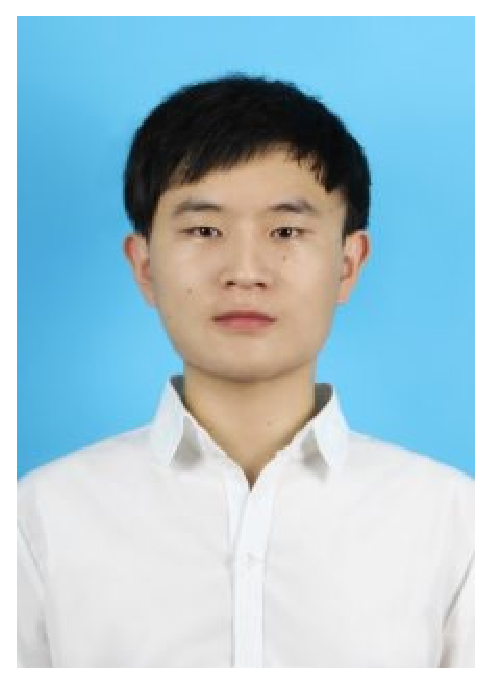
\includegraphics[width=1in,height=1.25in,clip,keepaspectratio]{ZhiqiangLiu.eps}}]{Zhiqiang Liu}
received the B.S degrees in electrical engineering from University of Science and Technology of China, Hefei, Anhui, China, in 2013, and he is currently pursuing the Ph.D. degree in electrical engineering from University of Science and Technology of China. His research interests lie resource allocation, energy-saving and Quality of Service guarantee in wireless body area networks. 
\end{IEEEbiography}%
\vspace{-20em}
\begin{IEEEbiography}[{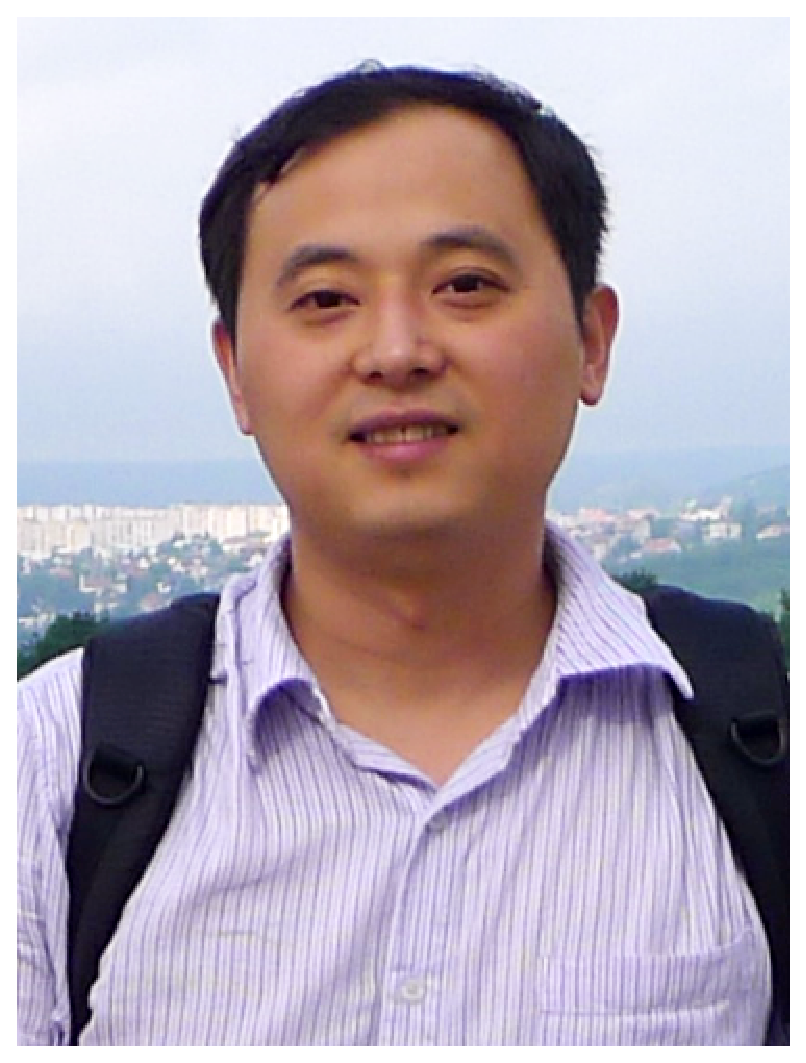
\includegraphics[width=1in,height=1.25in,clip,keepaspectratio]{BinLiu.eps}}]{Bin Liu}
received the B.S. and M.S. degrees, both in electrical engineering, from University of Science and Technology of China, Hefei, Anhui, China, in 1998 and 2001, respectively, and the Ph.D. degree in electrical engineering from Syracuse University, Syracuse, NY, in 2006. Currently, he is an Associate Professor with the School of Information Science and Technology, University of Science and Technology of China. His research interests are signal processing and communications in wireless sensor and body area networks.
\end{IEEEbiography}%
\vspace{-20em}
\begin{IEEEbiography}[{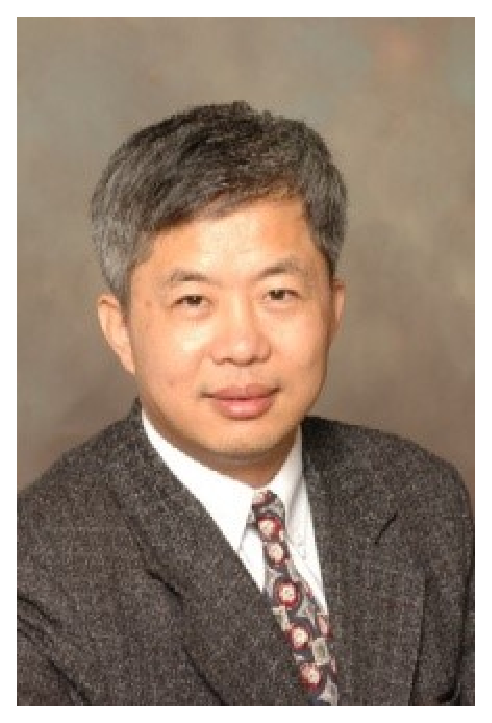
\includegraphics[width=1in,height=1.25in,clip,keepaspectratio]{ChangwenChen.eps}}]{Chang Wen Chen}
   (F'04) is a Professor of Computer Science and Engineering at the State University of New York at Buffalo, USA. Previously, he was Allen S. Henry Endowed Chair Professor at Florida Institute of Technology from 2003 to 2007, a faculty member at the University of Missouri - Columbia from 1996 to 2003 and at the University of Rochester, Rochester, NY, from 1992 to 1996. He has been the Editor-in-Chief for IEEE Trans. Multimedia since 2014. He has also served as the Editor-in-Chief for IEEE Trans. Circuits and Systems for Video Technology from January 2006 to December 2009 and an Editor for Proceedings of IEEE, IEEE TMM, IEEE JSAC, IEEE JETCAS, and IEEE Multimedia Magazine. He and his students have received eight (8) Best Paper Awards or Best Student Paper Awards and have been placed among Best Paper Award finalists many times. He is a recipient of Sigma Xi Excellence in Graduate Research Mentoring Award in 2003, Alexander von Humboldt Research Award in 2009, and SUNY-Buffalo Exceptional Scholar - Sustained Achievements Award in 2012. He is an IEEE Fellow and an SPIE Fellow. 
\end{IEEEbiography}%
 


% You can push biographies down or up by placing
% a \vfill before or after them. The appropriate
% use of \vfill depends on what kind of text is
% on the last page and whether or not the columns
% are being equalized.

%\vfill

% Can be used to pull up biographies so that the bottom of the last one
% is flush with the other column.
%\enlargethispage{-5in}



% that's all folks
\end{document}


